\documentclass[fleqn]{article}

\makeatletter
\newcommand{\vo}{\vec{o}\@ifnextchar{^}{\,}{}}
\makeatother
\usepackage[utf8]{inputenc}
\usepackage{amsmath}
\usepackage{amssymb}
\usepackage{graphicx}
\usepackage{hyperref}
\usepackage[section]{placeins}

\title{COMS3007A\\Machine Learning\\Assignment}
\author{Gideon Ilung \\ 2241186 \\ \\ Mpendulo Nxumalo}
\date{May-June 2021}

\begin{document}
	\maketitle
	\newpage
	
	\section*{Description of Dataset}
	
		\subsection*{Source of dataset}
			
			the dataset was retrieved from the following link: \\
			\url{https://www.kaggle.com/arashnic/covid19-hospital-treatment}\\
			\\the data was collected from multiple hospitals during the breakout of 				the pandemic (march 2020) till recently (May 2021).The data was collect 				so that predictions may be made to determine how long an individual may 				spend in hospital if they are hospitalised due to Covid 19.\\
			
		\subsection*{Summary of the Dataset}
			 The dataset consists of 318438 records and 18 features. \\
			 \\ the features being \\
			 \begin{itemize}
			 	\item case id 
			 	\item Hospital
			 	\item Hospital type
			 	\item Hospital city
			 	\item Hospital region
			 	\item Available Extra Rooms in Hospital
			 	\item Department
			 	\item Ward Facility
			 	\item Bed Grade
			 	\item patient id
			 	\item City Code Patient
			 	\item Type of Admission
			 	\item Illness Severity
			 	\item Patient Visitors
			 	\item Age
			 	\item Admission Deposit
			 	\item Stay Days
			 \end{itemize} 		 
			the target in this dataset will be Stay Days. the patient id and case id 			will not be used in the analysis and predict on the dataset, as it does 				not have much significance 
			
		\subsection*{Target: Stay Days}
			
			the target Stay Days consists of the following possible values:\\
			
			\begin{itemize}
				\item 0-10
				\item 11-20
				\item 21-30
				\item 31-40 
				\item 41-50
				\item 51-60
				\item 61-70
				\item 71-80
				\item 81-90
				\item 91-100
				\item More than 100 Days   
			\end{itemize}
			
			each representing a time frame in which a patient hospitalised will 					recover. death is not included as the data was collect on individuals 					who were hospitalised and survived covid 19.\\
			\\plotting the data we obtain Figure~\ref{fig:1} and Figure~\ref{fig:2}\\			
			\begin{figure}[hb]
  				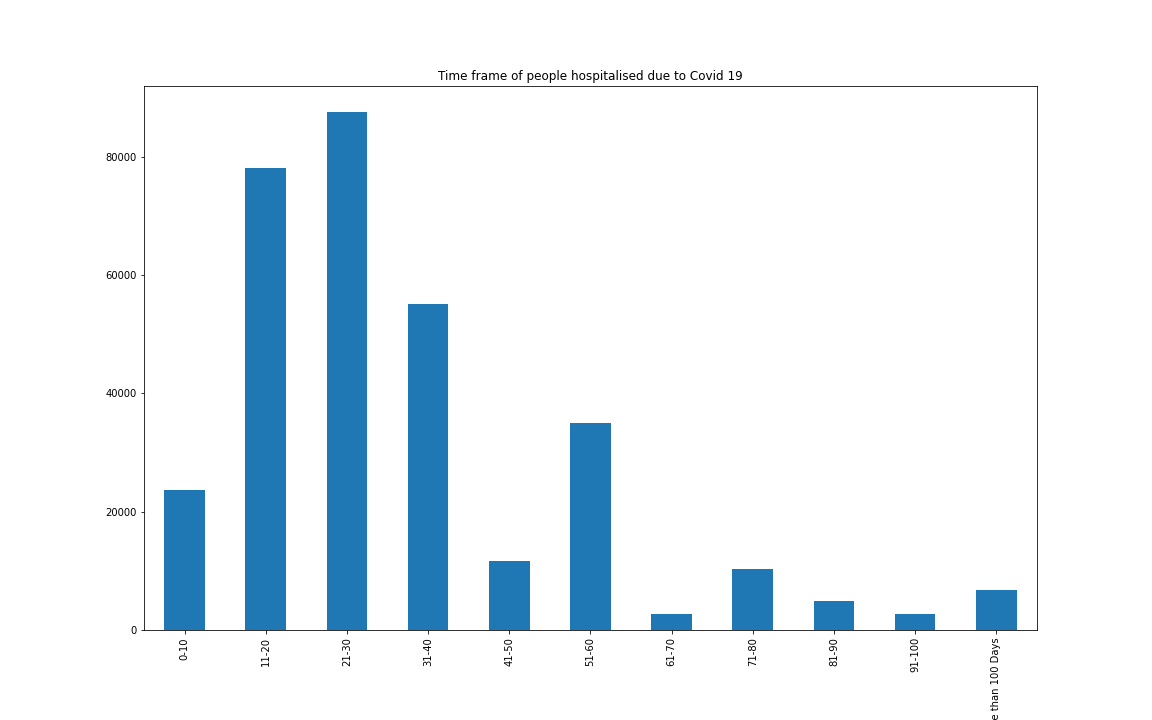
\includegraphics[width=\linewidth]{clas_hist.png}
  				\caption{Histogram of the number of people that stayed in each time 						frame}
  			\label{fig:1}
			\end{figure}
			\FloatBarrier
			\begin{figure}[hb]
  				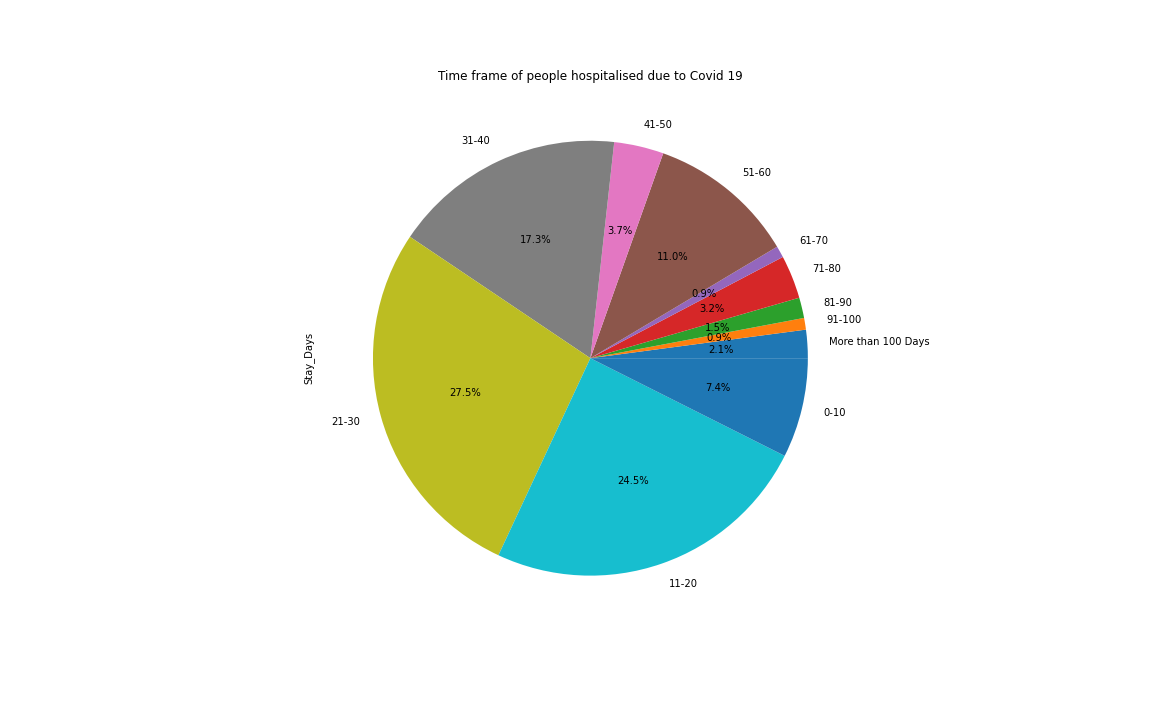
\includegraphics[width=\linewidth]{class_pie.png}
  				\caption{Pie chart of the number of people that stayed in each time 						frame}
  				\label{fig:2}
			\end{figure} 
			\FloatBarrier
			
			analysing the diagrams the following insights may be concluded: \\
			50 percent of people recover within 0-30 days of contracting the virus.
			which agrees with the medical experts opinion on the recovery time frame 			of Covid 19.
			
		\newpage
		\subsection*{Hospital}
			this feature gives information on which hospital the person was treated.
			plotting the results we obtain \\ 
			\begin{figure}[hb]
  				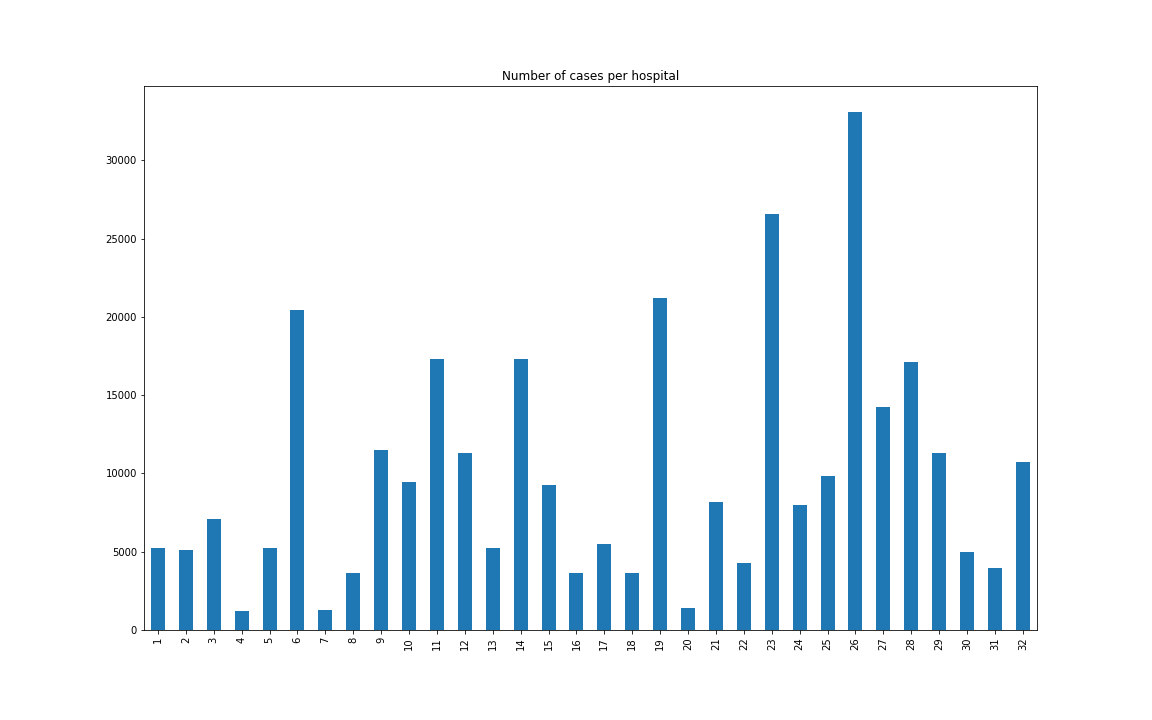
\includegraphics[width=\linewidth]{hospital_hist.png}
  				\caption{histogram showing how many cases were handled in each 							hospital}
  				\label{fig:3}
			\end{figure} 
			\FloatBarrier
			from this figure we can see majority of the cases were handled by 						Hospital 26. this may be due to numerous factors, to list them they 					could be due to the population density near the hospital and the cost of 			services.
		
		\newpage
		\subsubsection*{Hospital Type}
			this feature gives a discription of the type of hospital that treated 					the case. when plotting this data we obtain the following figure: \\
			\begin{figure}[hb]
  				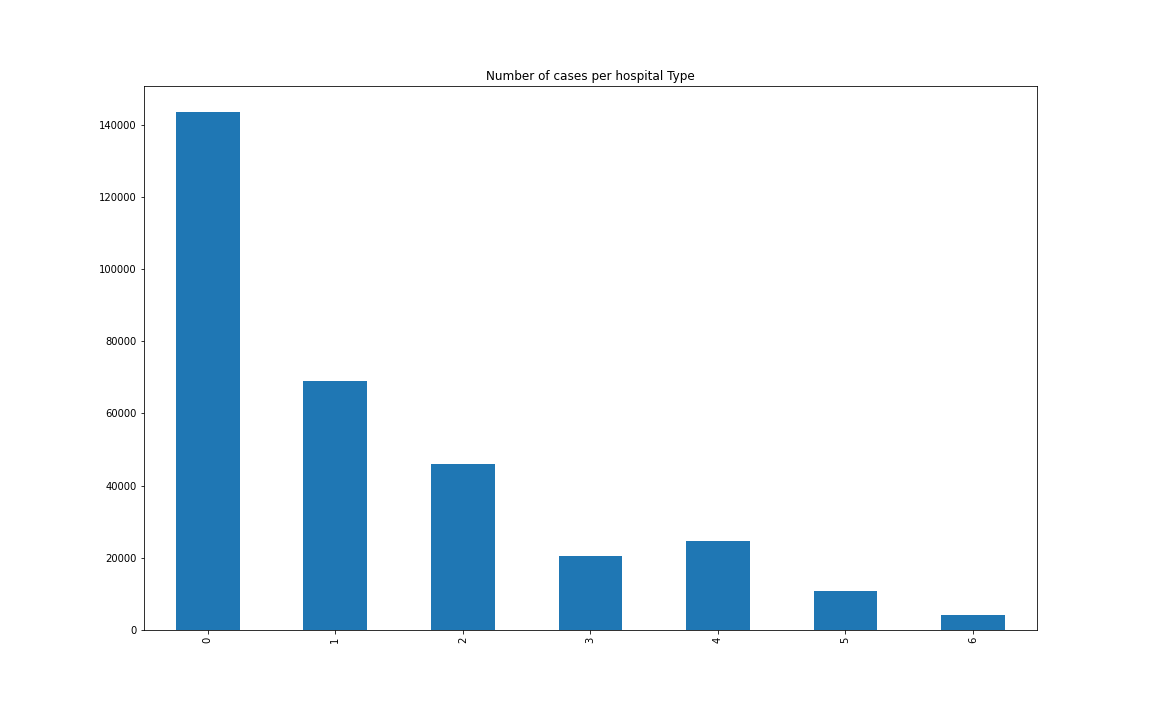
\includegraphics[width=\linewidth]{hospitalType_hist.png}
  				\caption{histogram showing how many cases were handled in each type 						of hospital}
  				\label{fig:4}
			\end{figure} 
			\FloatBarrier
			
			hospital type 0 handled the majority of the cases
			
		\subsection*{Hospital City}
		(find out what to add here)
		
		\subsection*{Hospital region}
		(find out what to add here)
		
		\subsection*{Available Extra Rooms in Hospital}
			this feature gives an indication on how many extra rooms the hospital 					where the patient was admitted has. when plotting the data we obtain the 			following graph:
			
			\begin{figure}[hb]
  				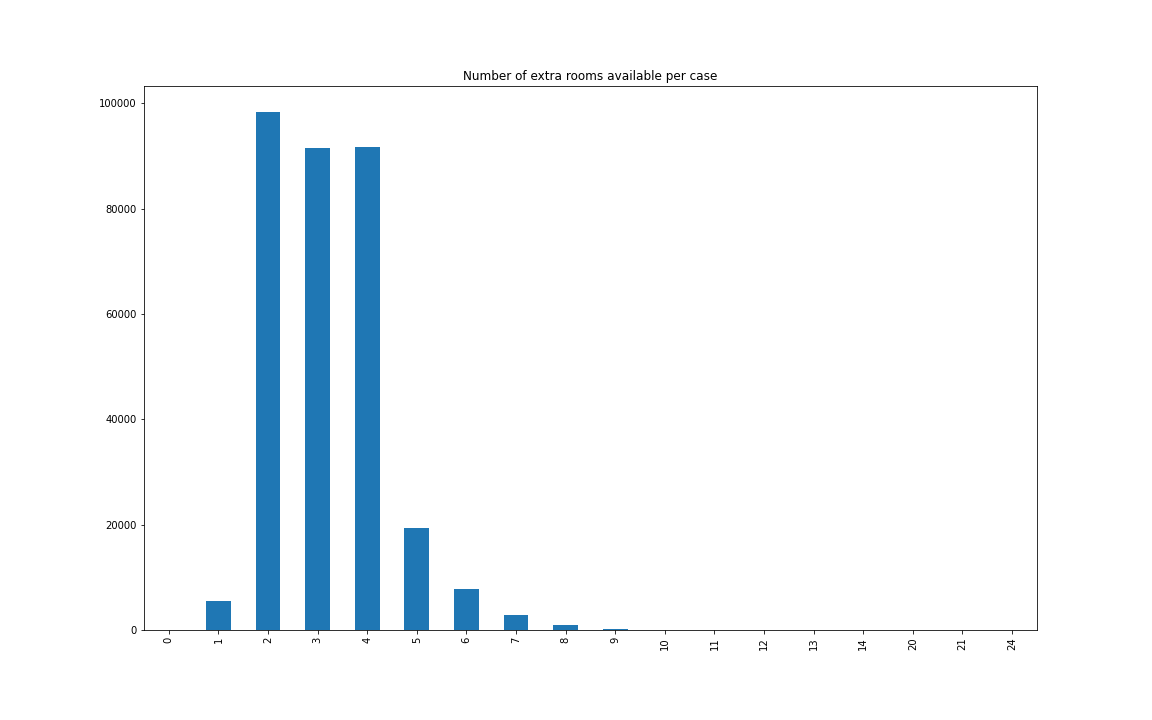
\includegraphics[width=\linewidth]{Extraroom_hist.png}
  				\caption{histogram showing how many rooms where available at time 						patient admitted}
  				\label{fig:5}
			\end{figure} 
			\FloatBarrier
			
			analysing the figure we may conclude that on average when a person was 					admitted to the hospital there was on average between 2-4 extra rooms 					available
			
		\subsection*{Department}
			this feature gives an indication in which department handled the case in 			the hospital. plotting this data we obtain the following figure:
			
			\begin{figure}[hb]
  				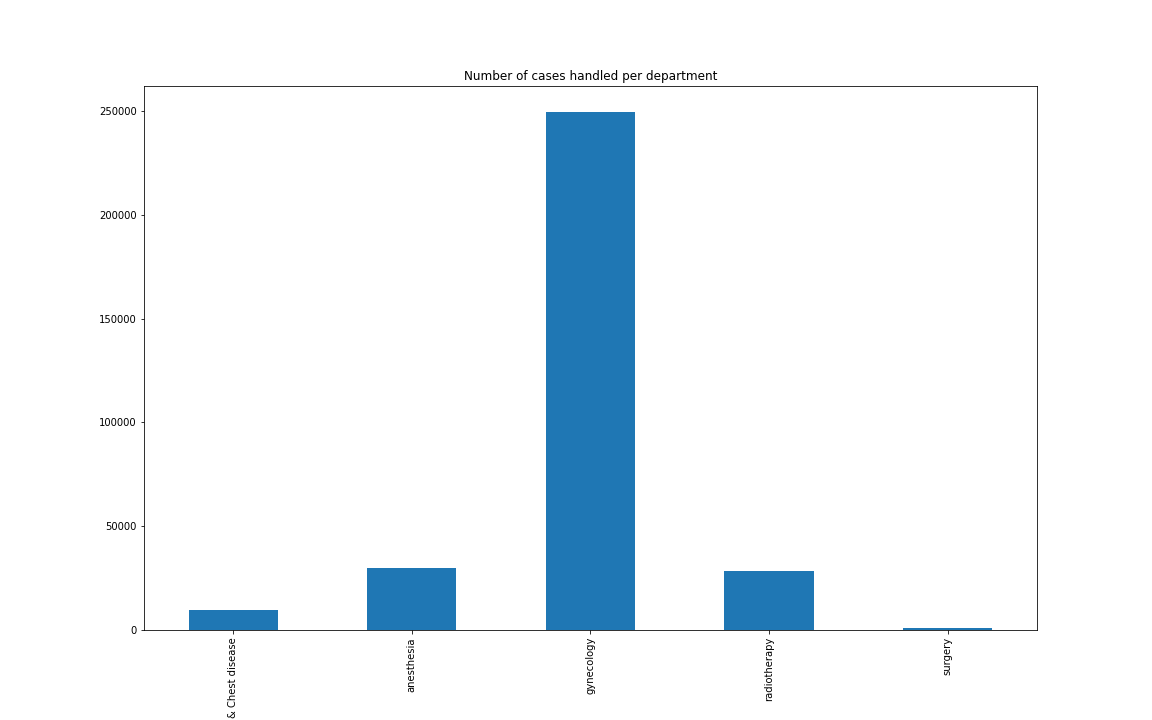
\includegraphics[width=\linewidth]{department_hist.png}
  				\caption{number of cases handled by each department}
  				\label{fig:6}
			\end{figure} 
			\FloatBarrier
			
			as seen in the figure above the department of gynecology handled an 					extreme huge proportion of the cases. this may be due to the availabilty 			of the staff assigned to that department, covid cases were spiking so 					getting any medical help would of made sense
			
			
		\subsubsection*{Ward Facility}
		 this feature gives an indication on how many cases were treated in each 				ward type plotting the data we obtain the following figure:
		 
		 \begin{figure}[hb]
  				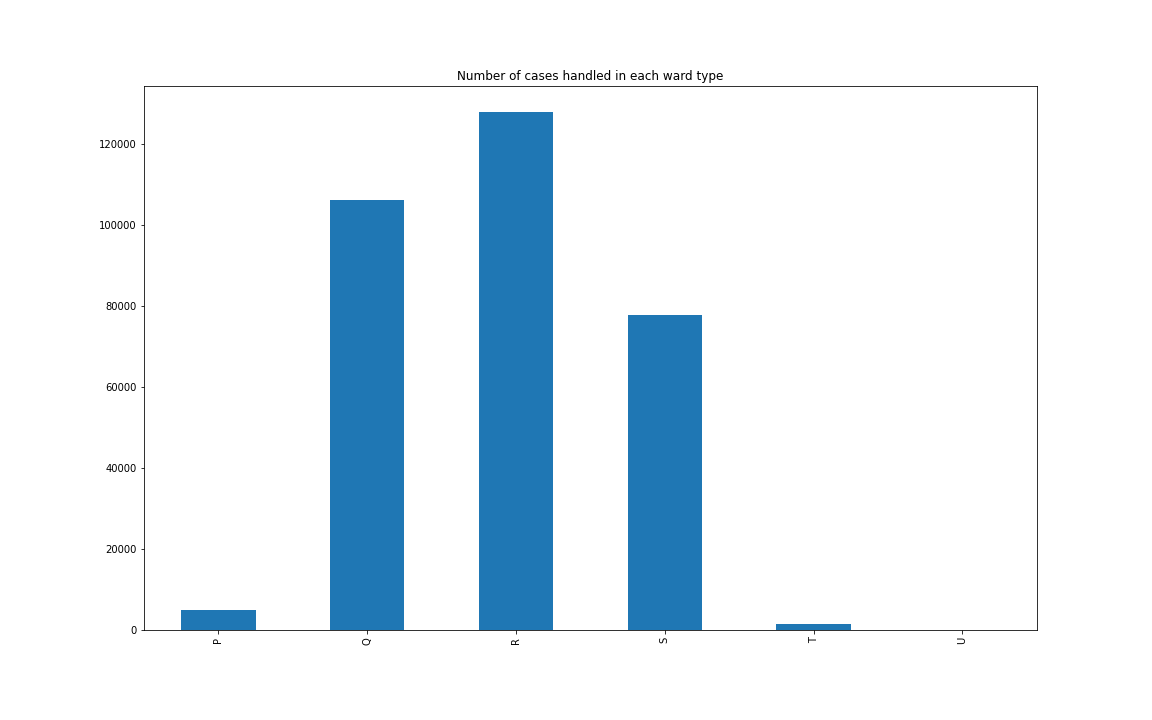
\includegraphics[width=\linewidth]{ward_hist.png}
  				\caption{number of cases handled by each ward type}
  				\label{fig:6}
			\end{figure} 
			\FloatBarrier
			
		as seen in the figure above ward type R handled majority of the cases. this 			may be due to the resources allocated to that ward type such as stuff, 					medicine etc
		
		\subsection*{Bed Grade}
			this feature gives us an idication on the quality of the beds used and 					the quantity of each type that was used. plotting this data we obtain 					the following figure:	
			
			 \begin{figure}[hb]
  				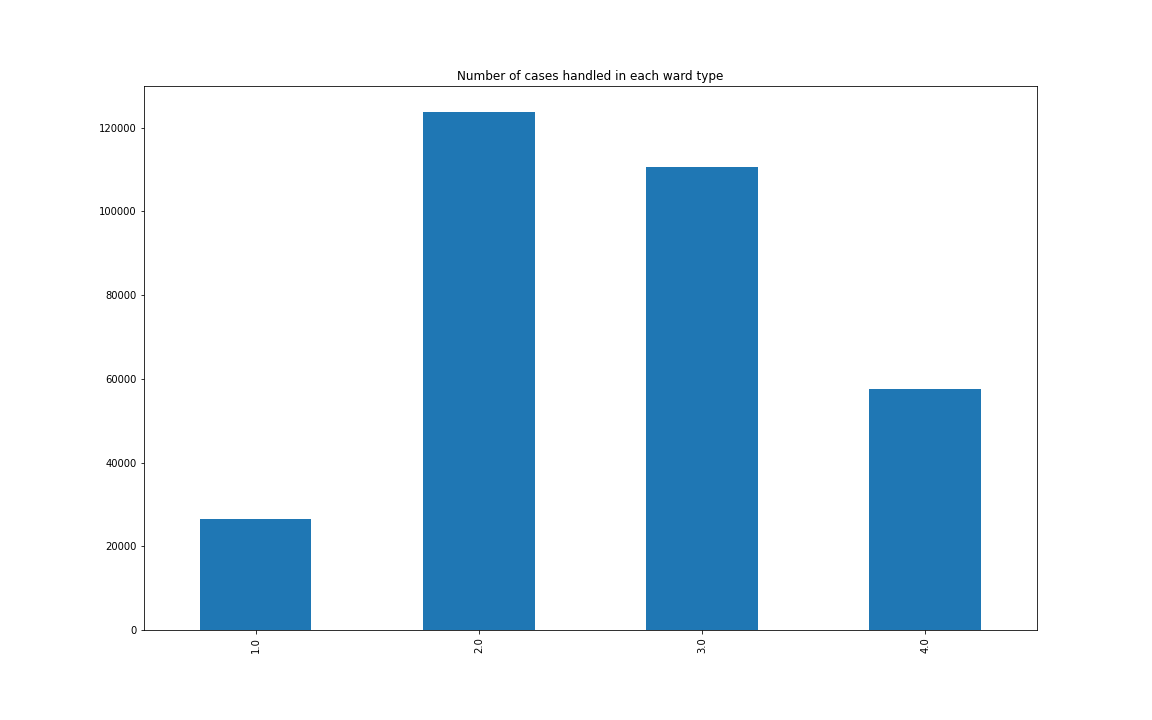
\includegraphics[width=\linewidth]{bed_hist.png}
  				\caption{number of beds assigned to patients of each grade}
  				\label{fig:6}
			\end{figure} 
			\FloatBarrier	
			
			from the figure above its clear that average beds were used majority of 				the time. this my be due to the financial strain brought by covid 19.
			
			
		\subsection*{Type of Admission}
			this feature describes the sense of urgency required for this case. 					plotting the data we obtain the following figure
			
			\begin{figure}[hb]
  				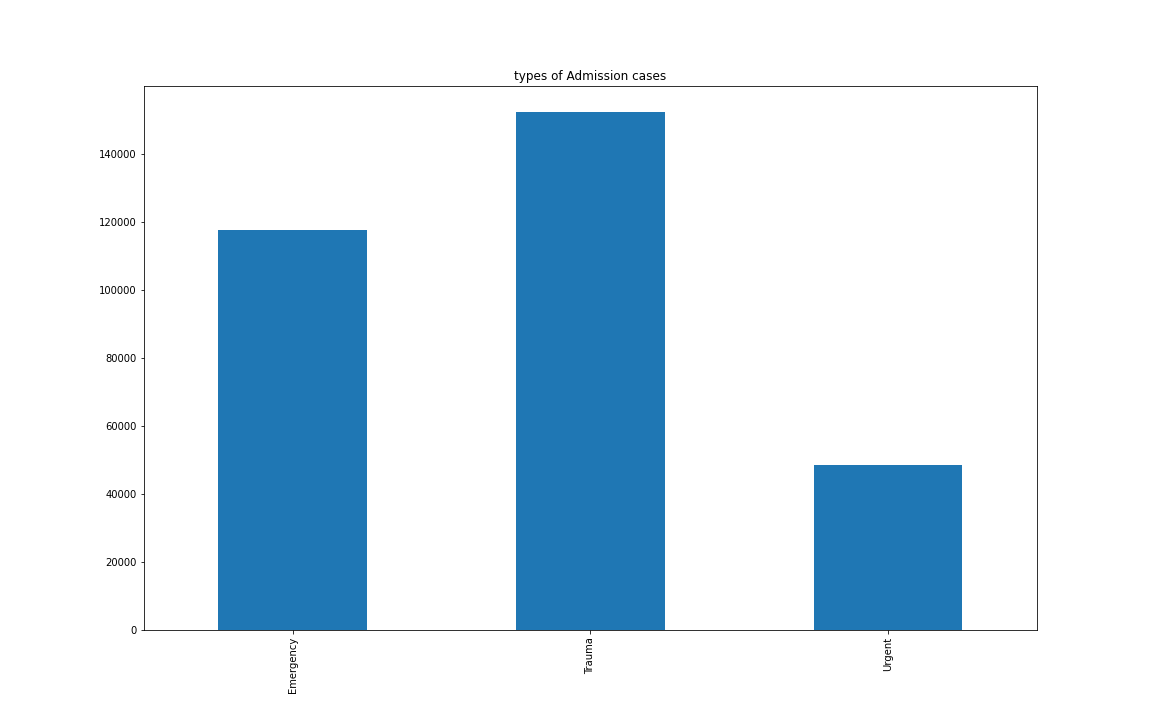
\includegraphics[width=\linewidth]{admin_hist.png}
  				\caption{types of Admission cases}
  				\label{fig:6}
			\end{figure} 
			\FloatBarrier
			
			as seen from the figure above majority of cases were considered trauma 					cases. this makes sense as for someone to be admitted to hospital due to 			covid 19 the patient is probably experiencing servere symptoms.
\end{document}